\documentclass[a4paper,11pt]{article}

\usepackage[affil-it]{authblk}
%\usepackage{amsfonts, amsmath, amssymb, bm}
%\usepackage{float}
\usepackage[margin=1.0in]{geometry}
\usepackage{graphicx}
%\usepackage{hyperref}
%\usepackage{subcaption}
%\usepackage{subfigure}
\usepackage{url}

%\graphicspath{{../pdf/}{../jpeg/}}
% \DeclareGraphicsExtensions{.pdf,.jpeg,.png}
\graphicspath{{figures/}}

%\newcommand{\bfnull}{\textbf{null}}

\begin{document}

\title{Towards the Planning of World Domination}
\author{Jason Gregory, Moshe Katz, \& Kamruzzaman Quddus \\ \{jgregory,mmkatz, kquddus\}@umd.edu}
\affil{University of Maryland, College Park, MD}
\date{\today}

\maketitle

%
\abstract{Abstract goes here.}

\section{Introduction}\label{sec:intro}
\subsection{AI in Games}\label{aiingames}
Although there are many major commercial fields which benefit from improvements
in Artificial Intelligence, one of the largest research areas in the field is
AI's application to games.  From the 1951 debut of Artificially Intelligent bots
for Nim \cite{nim}, checkers, and chess \cite{checkerschess}, to Deep Blue's 1997
defeat of chess grandmaster Garry Kasparov, and continuing to today's sophisticated
First-person-shooter adversaries, the impact and importance of AI in gaming as a
tool for understanding and furthering AI techniques for the real world has cannot
be overstated.

Despite all of this work, there still remain many "open problems" in game AI
design.  Many games still use AI bots that are quite naive, and some games have
not yet been determined to be winnable by a computer player. To encourage continued
research and development of game AI, some game makers occasionally run competitions
for developing new AI bots to play their games.

We are developing a bot to compete in the Warlight AI Challenge 2 \cite{warlight}.
The goal of this competition is to build a bot that can play (and, of course, can
win) Warlight, a RISK-style game.

\subsection{Problem Statement}\label{sec:problem}
We are developing an AI planner for the Warlight AI Challenge 2.  To aid those who
are already familiar with RISK, we first describe the gameplay mechanics of 
RISK,\footnote{While a full description of the rules of RISK would be too long to 
include here, the basics described should be enough to understand the general 
gameplay.  The reader is directed to the printed rules document found in the game 
box for additional details.} then the differences of Warlight.

\subsubsection{RISK}
At the start of a game, players take turns placing troops on the board to claim
their territories.  After all territories have been claimed, players place
additional troops on the board, with the number of additional troops depending on
the number of game players.  All players choose the same number of territories.
When only two players are playing, as is the case in the games our bot will play,
one third of the territories remain neutral, which means that they will only defend
against attacks from the two players, but they will not attack on their own.

At the beginning of every turn, players receive additional armies to place on the 
game board.  The number of armies varies based on how many territories the player 
controls, and includes additional bonus armies if the player controls entire 
continents or if the player plays any "RISK Cards".  Players place these armies 
before continuing their turns.  The rest of 
a player's turn consists of attacking neighboring territories held by opposing 
troops and/or transferring troops to a neighboring territory held by the player's 
own troops in order to fortify it. (Only one fortification move may be made per 
turn, and it must be the last move of the turn.)

When a player attacks another player's territory, the attacker rolls a number of 
dice, as does the defender.  The dice are compared and the loser of each comparison 
removes an army token from the territory.  The attacker conquers the territory if 
the defender's last army is removed from it, in which case the attacker must move 
some of his troops into the attacked territory.  The attacker also draws a "RISK 
Card" which can be traded-in in a set of three on a future turn to receive more 
troops.

\subsubsection{Warlight}
Warlight has several modifications from the RISK gameplay.  The most significant 
change is the addition of \textbf{fog of war}, meaning that players can only see 
their own territories and the territories immediately adjacent to them.  
Additionally, while RISK is played on a world map that has been divided into 
(largely arbitrary) territories, Warlight can also be played on custom-designed or 
randomly-generated maps.  Warlight also has many additional types of cards that can 
be drawn, including Reinforcement cards (like RISK), Blockade cards, Spy and 
Surveillance cards, Gift cards, and several other types.

A major factor in developing a strategy for playing Warlight is that a multi-player 
(human) Warlight game may have many configurable options set by the game host - 
this makes developing a strategy that covers all game options impossible. Because 
RISK is usually played on a physical game board, the per-game options are limited 
to simple "house rules" modifications; for this reason, there are many published 
RISK strategy guides but but very few guides for Warlight (and guides for Warlight 
are usually much more vague about specific implementation of the strategies 
discussed therein \cite{warlightguide}).

\subsubsection{The Warlight AI Challenge 2}
For the Warlight AI Challenge 2, our bot will play a two-player game against 
another bot.  The game will be played on a random map, using the standard scoring 
and troop allocation rules, but not using any cards.

One major game setting is called the \textbf{luck factor}. The luck factor is used 
in the calculation of how many attacking and defending armies are destroyed.  While 
the previous Warlight AI Challenge used a luck factor of 100\%, this challenge uses 
only 16\% so there is a lot less luck and a lot more certainty about the outcome of 
an attack.

A bot wins the game by destroying all of the armies of the opposing bot.  However, 
if the turn limit of the game is reached, the game is considered a draw.  The 
maximum number of turns allowed in a game depends on the size of the map, and is 
currently set as the number of map regions times 2.5.

\subsection{Previous Work}\label{sec:previous}

There are currently around 200 competition entries from 30 countries written in 
eleven languages \cite{warlight}.  While we have not yet examined any of our competitors in detail, 
they are all working toward the same goal as we are of developing an AI bot for 
this game, and many of them are much farther ahead at this time.

Additional related work comes from the first Warlight AI Challenge.  While the 
rules of the game for that competition were slightly different, many of the 
techniques used there will still apply to this challenge, either as examples of 
successful approaches, or otherwise as examples of what not to try.

There are also many strategy guides that exist for RISK.  However, as discussed 
above, there is no real complete strategy guide for Warlight.  Given that every 
game our bot will be playing will be on a completely new random map, many of the 
normal things found in any strategy guide might not apply to every game, especially 
the static RISK guide.  Additionally, many common RISK strategies require knowledge 
of more of the board status than Warlight allows us to have (due to fog of war).

Finally, there are existing AI bots for RISK itself.  While some have been 
discussed only theoretically, including strategies from MIT \cite{riskmit}, Markov 
Chains from North Carolina State University \cite{riskncs}, Monte-Carlo (UCT) 
techniques for territory selection from University of Alberta \cite{riskalb}, and 
studies of dice-rolls from Elon University \cite{riskelon}, implementations of AI 
players for RISK have been created an sold in commercial software as early as 1989.  
While these are also of varying quality - the 1992 release of \textit{WinRisk} for 
Windows 3.1 was capable of beating an inexpert child player, but not so easily 
playing against an expert - and most of them are closed-source without any 
documentation of their algorithms, they are still prior work for creating an AI bot 
that can play RISK and similarly-structured games.

\subsection{Importance and Relevancy}\label{sec:importance}
In addition to the obvious goal of winning the AI Challenge, we will use this
project as a mechanism to learn and practice topics from class and demonstrate
applying them to a real-world use-case.

Moreover, techniques used for tactical gameplay often have further real-world 
application for training exercises and simulations of real situations.  This is 
especially true for algorithms that model adversarial behavior in addition to our 
own, providing the ability to play out WarGames-style dangerous scenarios in 
complete safety.\footnote{In fact, the NORAD missile command center was already 
using the RISK-style AI shown in WarGames in 1979, and there really was an incident
in which the AI simulation was thought to be a real Soviet attack
\cite{wargamesreal}.}

%
\section{Technical Approach}\label{sec:approach}
Our approach for designing a planner for the Warlight AI Challenge 2 is to implement the basic UCT algorithm and then, time permitted, improve the performance of the algorithm by making different modifications.


\subsection{Hypothesis}\label{sec:hypothesis}
We believe that the Monte Carlo-based UCT algorithm will enable the search of different applicable moves in the fast-paced, time-limited game of the Warlight AI Challenge 2. We also hypothesize that, due to the strict time constraint enforced by the game engine, we will be required to modify the UCT algorithm to expedite the search through the game tree.  By making these modifications, we feel that we can make intelligent decisions in each turn that eventually lead to winning the game.

\subsection{Process}\label{sec:process}
The general strategy for the planning algorithm is to acquire regions in a manner by which power is gained quickly while always remaining tactically flexible so as to starve the opponent from in-game advantages. Such a planner must be adversarial in nature, robust enough to adapt to different counter strategies, efficient enough to plan quickly, and adhere to the constraints defined by the games rules.

The various constraints in the Warlight AI Challenge 2 primarily dictate how we will approach developing a planner. First, the game provides each player with a $10$ second timebank that ultimately limits one from planning extensively in each turn.  Additionally, this game increases the difficulty of the original Risk game by introducing the concept of fog of war - that is, a player can only observe regions that are immediately adjacent to their own regions. This incorporates a level of uncertainty into the game that must be met with a probabilistic planner instead of a deterministic one. As a result of these constraints imposed by the game engine, we desire an algorithm that balances planning performance with run time; otherwise, we will run out of time, never make a move, and lose the game. 

From our research, classical planning techniques that exhaustively explore the entire state space are not applicable to this problem because of the time required to find an optimal plan. Instead, we propose to use the Monte-Carlo-based UCT algorithm.  First, we plan on implementing the basic UCT algorithm so that we can generate a sensible plan each turn for a single region in our possession.  Next, we plan to extend this implementation so that we will execute a new instance of the UCT algorithm for every region that contains more than one of our troops.  In other words, regions that we own and have the ability to attack or transfer will have separate game trees. We will simulate the game for each game tree simultaneously using threads, initially disregarding any time constraint, and produce a set of the best moves, each with some probability $p_{i}$. Note, due to the nature of the UCT algorithm, we will not produce an optimal solution, but rather a solution with a certain probability of success, which we can apply some metric to determine the quality of the plan of actions. We believe we are able to evaluate each region independently because the attack and transfer commands in a game are independent. We plan to initially evaluate the UCT algorithm without enforcing a time constratint so that we can characterize the performance of the algorithm completely and determine an upper bound for the run time required to produce all possible commands. 

Depending on the amount of time required to traverse the entire game tree in a single instance of the UCT algorithm, we may be required to implement some methods for speeding up the search. One possible method we are considering is the concept of a zone for the purposes of more efficient simulation generation.  We define a zone to be a collection of regions where each region is a neighbor to at least one region with the same owner and at least one region with an opposing owner.  From this definition we can develop a strategy for quickly identifying whether it is intelligent to attack an opponent by comparing the total number of troops in our zone versus the opponent's zone.  In the event an attack is not advised, substantial processing time will be saved by reducing the instances of the UCT algorithm.  An additional modification we are contemplating, provided there is sufficient time in the semester, is the incorporation of a minimax approach to evaluate our moves and the opponent's moves.  Also, we may try prioritizing actions based on the probability of success, prioritizing certain events that may lead to more promising future moves consistent with our strategy, and different thresholds for limiting the depth in which UCT explores a game tree. The specific details of these modifications will be determined during our development and testing tasks.

In terms of evaluation, we will simulate several different approaches that incorporate as many modifications as time permits.  Each solution will be simulated in a large number of trials, each in a randomly generated map, and then the performance will be assessed based on the number of games won as well as the rate at which the game was won.  In this case, the rate of winning a game is defined as the number of rounds required to win divided by the total number of rounds in the game. The Warlight AI Challenge 2 also provides a leaderboard that indicates the user's with the best performing algorithms. At a high-level We plan to compare the performance of our approach with the leaders in the challenge.

Hypothetically, the proposed approach could produce largely varied results and is possibly dependent on the size of the map or the complexity of the opponent's algorithm. We seek to characterize the overall performance as it relates to these potential dependencies.  Our analysis and findings will be detailed in final report and presentation.

%Essential elements such as parsing routines as sensor/actuator platform will generate commands for the engine, events, create/update sate variables and possibly some book-keeping resources such as look-up tables (to be used by probabilistic routines) will also need to be developed. State variables, tasks and events will work as the  communication scheme between each level of this hierarchical adversarial planner.


%
\section{Project Management}\label{sec:management}
The main tasks for this project include implementing the UCT algorithm, conducting simulations, and evaluating the generated data so that we can publish our results in a report and a presentation. 

\subsection{Tasks}\label{sec:tasks}
There are seven main tasks required to successfully develop a planner that is capable of winning a game in the Warlight AI Challenge 2.  The first, which we have already completed, is a literature review of the UCT algorithm, its variants, and its application to the planning of games involving artificial intelligence. The next task is formulating the problem in a manner that is compatible with our proposed approach. With a concrete understanding for a possible solution, the next task is to implement the basic UCT algorithm.  The next two tasks consist of testing, modifying and improving our implementation to enhance the performance of our solution.  A simulation and evaluation of our algorithm is required to determine how well it performs compared to other strategies. Finally, we will present our results in a report and a presentation.  These tasks, with their respective tentative target dates and durations are summarized in Table~\ref{tab:deadlines}.

%
\begin{table}[htbp]
  \centering
  \begin{tabular}{|c|c|}
    \hline
    \emph{Task} & \emph{Target Date} \\ 
    \hline
    Literature Review & March 9, 2015 \\ \hline
    Problem Formulation & March 16, 2015 \\ \hline
    UCT Implementation & April 6, 2015 \\ \hline
    Testing & April 13, 2015 \\ \hline
    UCT Modification and Improvement & April 13, 2015 \\ \hline
    Simulation and Evaluation & April 27, 2015 \\ \hline
    Write Report and Presentation & May 2, 2015 \\ \hline
  \end{tabular}
  \caption{Table of project tasks and target dates for completing each task.}
  \label{tab:deadlines}
\end{table}
%

\subsection{Assignments}\label{sec:assignments}
All three group members will be responsible for contributing to the problem formulation. This ensures that everyone in the group fully understands both the problem at hand and the proposed solution.  Jason Gregory and Kamruzzaman Quddus will work together to implement the proposed UCT algorithm and its modifications.  Moshe Katz will incrementally test the team's implementation as the code is being written to ensure correct functionality and then collect data by executing numerous simulations. The group, as a whole, will collaboratively evaluate the result, develop a thorough analysis, and create the paper and presentation.


\subsection{Schedule}\label{sec:schedule}
Figure~\ref{fig:schedule} presents our tentative schedule for completing this project during the 2015 Spring semester. Note that we intend on testing our implementation as we develop it so that we can parallelize our efforts and have more time for simulation and evaluation.

%
\begin{figure}[htbp]
  \centering
  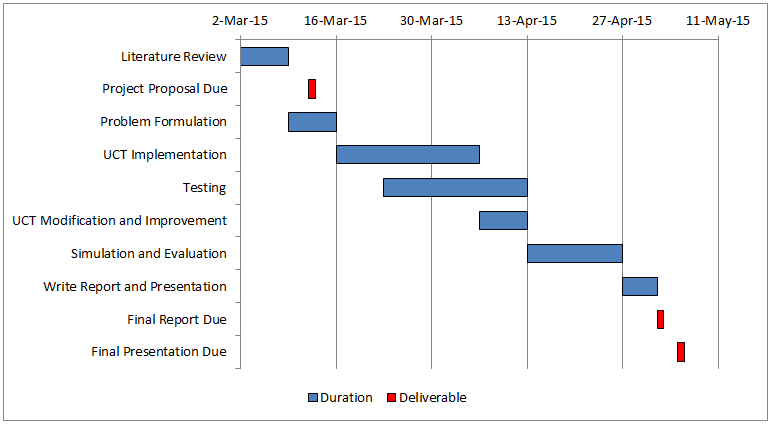
\includegraphics[width=0.95\columnwidth]{gantt_chart}
  \caption{Tentative schedule for completing each task. Note, red boxes indicate deliverables that will be submitted to the professor.}
  \label{fig:schedule}
\end{figure}


%
\section{Conclusions}\label{sec:conclusions}
In this proposal we present our anticipated efforts for developing a probabilistic planner whose goal is to consistently win games in the Warlight AI Challenge 2. On the surface, this toy problem may appear to have little value as it seems inapplicable to real-world problems; however, upon further analysis one immediately sees the expected contributions from our technical approach.  To our knowledge, this will be the first appliation of the UCT algorithm to Risk and its variant Warlight. 

% References 
\bibliographystyle{plain}
\bibliography{references}

% End document
\end{document}
